\renewcommand{\nrandom}{\num{700}}
\renewcommand{\napplication}{\num{212}}
\newcommand{\ntoilet}{\num{77}}
\newcommand{\nmaxcount}{\num{26}}
\newcommand{\nsandcastle}{\num{25}}
\newcommand{\nconformant}{\num{24}}
\newcommand{\nmpec}{\num{60}}

\begin{frame}
    \frametitle{Evaluation}
    \begin{itemize}
        \item Compared solvers
              \begin{itemize}
                  \item \erssat: \texttt{C++} language inside~\abc~\cite{ABC}
                        \begin{itemize}
                            \item SAT solver: \minisat-2.2~\cite{Een2003Solver}
                            \item Weighted model counter: \cachet~\cite{Sang2004} and \cudd~\cite{Darwiche2002KnowledgeCompilation}
                        \end{itemize}
                  \item \erssatb: \erssat without heuristics to strengthen learnt clauses
                  \item \dcssat: state-of-the-art DPLL-based SSAT solver
              \end{itemize}
              \pause
        \item Experimental setup
              \begin{itemize}
                  \item A machine with~\machineSpec
                  \item \osInfo
                  \item CPU time: \timelimit; memory: \memlimit
              \end{itemize}
    \end{itemize}
\end{frame}

\begin{frame}
    \frametitle{Benchmark Set}
    \begin{itemize}
        \item Random $k$-CNF formulas (by \cnfgen~\cite{Lauria2017CNFgen})
              \begin{itemize}
                  \item $k\in\{3,\ldots,9\},n\in\{10,20,\ldots,50\},\frac{m}{n}=\{k-1,k,k+1,k+2\}$
                  \item Quantify half variables existentially and others randomly
                  \item \num{5} samples per configuration: \nrandom~formulas
              \end{itemize}
              \pause
        \item Application formulas: \napplication~formulas
              \begin{table}[ht]
                  \centering
                  \small
                  \begin{tabular}{c|c|c}
                      Family               & Description                                            & Number       \\
                      \hline
                      \textit{Toilet-A}    & Adapted from exist-forall QBFs~\cite{Narizzano2006}    & \ntoilet     \\
                      \textit{Conformant}  & Adapted from exist-forall QBFs~\cite{Narizzano2006}    & \nconformant \\
                      \textit{Sand-Castle} & A probabilistic planning problem~\cite{Majercik1998}   & \nsandcastle \\
                      \textit{Max-Count}   & Adapted from maximum model counting~\cite{Fremont2017} & \nmaxcount   \\
                      \textit{MPEC}        & Maximum probabilistic equivalence checking             & \nmpec       \\
                  \end{tabular}
              \end{table}
    \end{itemize}
\end{frame}

\begin{frame}
    \frametitle{Implications from the Results}
    \begin{itemize}
        \item \erssat performs similarly as \dcssat on random formulas
              \pause
        \item \erssat is not suitable for certain application formulas
              \begin{itemize}
                  \item Clause-containment learning might degenerate to brute-force search
                  \item Overhead incurred by the heuristics to strengthen learnt clauses
              \end{itemize}
              \pause
        \item \erssat is good at deriving tight lower bounds for large formulas
    \end{itemize}
\end{frame}

\begin{frame}
    \frametitle{Quantile Plot for Random Formulas}
    \begin{figure}
        \centering
        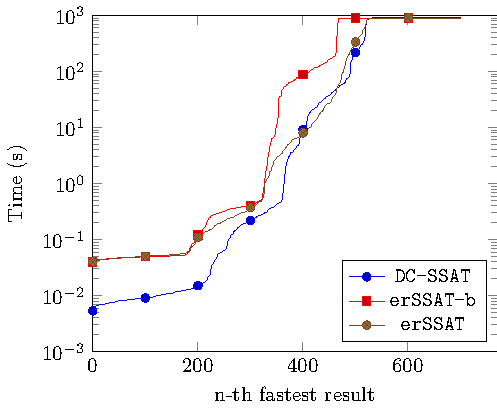
\includegraphics{fig/exist-random-ssat/quantile-cputime-Random.pdf}
    \end{figure}
\end{frame}

\begin{frame}
    \frametitle{Quantile Plot for Application Formulas}
    \begin{figure}
        \centering
        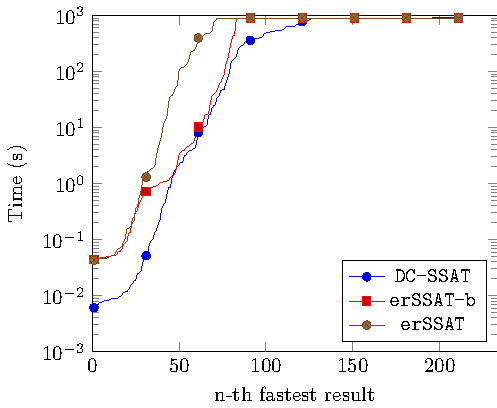
\includegraphics{fig/exist-random-ssat/quantile-cputime-Application.pdf}
    \end{figure}
\end{frame}

\begin{frame}
    \frametitle{Summary of Results for Application Formulas}
    % Commands for application formulas of ER-SSAT
\newcommand{\dcssatToiletA}{\num{44}}
\newcommand{\dcssatconformant}{\num{1}}
\newcommand{\dcssatcastle}{\num{21}}
\newcommand{\dcssatMaxCount}{\num{2}}
\newcommand{\dcssatMPEC}{\num{3}}
\newcommand{\erssatbToiletA}{\num{45}}
\newcommand{\erssatbconformant}{\num{1}}
\newcommand{\erssatbcastle}{\num{14}}
\newcommand{\erssatbMaxCount}{\num{1}}
\newcommand{\erssatbMPEC}{\num{1}}
\newcommand{\erssatToiletA}{\num{38}}
\newcommand{\erssatconformant}{\num{2}}
\newcommand{\erssatcastle}{\num{13}}
\newcommand{\erssatMaxCount}{\num{3}}
\newcommand{\erssatMPEC}{\num{2}}

    \begin{table}[t]
        \centering
        \begin{tabular}{l|ccc}
            \toprule
            Algorithm                              & {\dcssat}                                                     & {\erssat} & {\erssatb} \\
            \midrule
            Solved formulas                        & \num{\DcssatErDefaultApplicationMissingCount}
                                                   & \num{\ErssatDefaultBddApplicationMissingCount}
                                                   & \num{\ErssatBareBddApplicationMissingCount}                                            \\
            \qquad \textit{Toilet-A}               & \num{\dcssatToiletA}
                                                   & \num{\erssatToiletA}
                                                   & \num{\erssatbToiletA}                                                                  \\
            \qquad \textit{Conformant}             & \num{\dcssatconformant}
                                                   & \num{\erssatconformant}
                                                   & \num{\erssatbconformant}                                                               \\
            \qquad \alert<2>{\textit{Sand-Castle}} & \num{\dcssatcastle}
                                                   & \num{\erssatcastle}
                                                   & \num{\erssatbcastle}                                                                   \\
            \qquad \textit{Max-Count}              & \num{\dcssatMaxCount}
                                                   & \num{\erssatMaxCount}
                                                   & \num{\erssatbMaxCount}                                                                 \\
            \qquad \textit{MPEC}                   & \num{\dcssatMPEC}
                                                   & \num{\erssatMPEC}
                                                   & \num{\erssatbMPEC}                                                                     \\
            Timeouts                               & \num{\DcssatErDefaultApplicationErrorTimeoutCount}
                                                   & \num{\ErssatDefaultBddApplicationErrorTimeoutCount}
                                                   & \num{\ErssatBareBddApplicationErrorTimeoutCount}                                       \\
            Out of memory                          & \num{\DcssatErDefaultApplicationErrorOutOfMemoryCount}
                                                   & \num{\ErssatDefaultBddApplicationErrorOutOfMemoryCount}
                                                   & \num{\ErssatBareBddApplicationErrorOutOfMemoryCount}                                   \\
            Other inconclusive                     & \num{\DcssatErDefaultApplicationErrorOtherInconclusiveCount}
                                                   & \num{\ErssatDefaultBddApplicationErrorOtherInconclusiveCount}
                                                   & \num{\ErssatBareBddApplicationErrorOtherInconclusiveCount}                             \\
            \bottomrule
        \end{tabular}
    \end{table}
\end{frame}

\begin{frame}
    \frametitle{Case Study: \textit{Sand-Castle}}
    \begin{itemize}
        \item An agent wants to build a sand castle within finite stages
              \begin{itemize}
                  \item At each stage: either dig a moat or erect a castle
              \end{itemize}
              \pause
        \item Conformant planning: E-MAJSAT
              \begin{itemize}
                  \item Existentially quantified variables: policy selection
                  \item Randomly quantified variables: probabilistic mechanism
              \end{itemize}
              \pause
        \item Two-stage formula: $(\lnot d_1\lor \pf_d^{(1)})(\lnot e_1\lor \pf_e^{(1)})(\lnot d_2\lor \pf_d^{(2)})(\lnot e_2\lor \pf_e^{(2)})$
              \begin{itemize}
                  \item Dig at stage~$1$ and erect at stage~$2$: $\pf_d^{(1)}\land\pf_e^{(2)}$
                  \item Each policy selects a distinct set of clauses
                  \item Clause-containment learning degenerates to brute-force search
              \end{itemize}
              \pause
        \item \textit{Sand-Castle} favors \dcssat: same subformulas  across the stages
    \end{itemize}
\end{frame}

\begin{frame}
    \frametitle{Approximate E-MAJSAT Solving: \erssat on \textit{MPEC}}
    \begin{table}[ht]
        \centering
        \scriptsize
        \pgfplotstabletypeset[
            every head row/.style={before row={\toprule
                            & \multicolumn{4}{c}{\dcssat} & \multicolumn{8}{c}{\erssat}\\},after row=\midrule},
            every last row/.style={after row=\bottomrule},
            every row no 0/.style={before row={\rowcolor{yellow}}},
            every row no 8/.style={before row={\rowcolor{yellow}}},
            empty cells with={--},
            formula column/.list={0},
            time column/.list={1,3},
            prob column/.list={2,4},
            lbound column/.list={5},
            lbtime column/.list={6}
        ]
        {exist-random-ssat/parsed-MPEC-erssat.csv}
    \end{table}
\end{frame}